% !TEX TS-program = pdflatex
% !TEX encoding = UTF-8 Unicode

% This is a simple template for a LaTeX document using the "article" class.
% See "book", "report", "letter" for other types of document.

\documentclass[11pt]{article} % use larger type; default would be 10pt

\usepackage[utf8]{inputenc} % set input encoding (not needed with XeLaTeX)
\usepackage{dirtree}
\usepackage{graphicx}
%%% Examples of Article customizations
% These packages are optional, depending whether you want the features they provide.
% See the LaTeX Companion or other references for full information.

%%% PAGE DIMENSIONS
\usepackage{geometry} % to change the page dimensions
\geometry{a4paper} % or letterpaper (US) or a5paper or....
% \geometry{margin=2in} % for example, change the margins to 2 inches all round
% \geometry{landscape} % set up the page for landscape
%   read geometry.pdf for detailed page layout information

\usepackage{graphicx} % support the \includegraphics command and options

% \usepackage[parfill]{parskip} % Activate to begin paragraphs with an empty line rather than an indent

%%% PACKAGES
\usepackage{booktabs} % for much better looking tables
\usepackage{array} % for better arrays (eg matrices) in maths
\usepackage{paralist} % very flexible & customisable lists (eg. enumerate/itemize, etc.)
\usepackage{verbatim} % adds environment for commenting out blocks of text & for better verbatim
\usepackage{subfig} % make it possible to include more than one captioned figure/table in a single float
% These packages are all incorporated in the memoir class to one degree or another...

%%% HEADERS & FOOTERS
\usepackage{fancyhdr} % This should be set AFTER setting up the page geometry
\pagestyle{fancy} % options: empty , plain , fancy
\renewcommand{\headrulewidth}{0pt} % customise the layout...
\lhead{}\chead{}\rhead{}
\lfoot{}\cfoot{\thepage}\rfoot{}

%%% SECTION TITLE APPEARANCE
\usepackage{sectsty}
\allsectionsfont{\sffamily\mdseries\upshape} % (See the fntguide.pdf for font help)
% (This matches ConTeXt defaults)

%%% ToC (table of contents) APPEARANCE
\usepackage[nottoc,notlof,notlot]{tocbibind} % Put the bibliography in the ToC
\usepackage[titles,subfigure]{tocloft} % Alter the style of the Table of Contents
\renewcommand{\cftsecfont}{\rmfamily\mdseries\upshape}
\renewcommand{\cftsecpagefont}{\rmfamily\mdseries\upshape} % No bold!

%%% END Article customizations

%%% The "real" document content comes below...

\title{Technical Manual for the Personality Demonstrator}
\author{Robert Kraaijeveld, Cees-Jan Nolen, Steven Schenk}
%\date{} % Activate to display a given date or no date (if empty),
         % otherwise the current date is printed 

\begin{document}
\maketitle

\newpage
\tableofcontents
\newpage

\section{Introduction}
The application to which this manual is attached, the 'Personality Demonstrator', was made by the three authors of this document for their 3rd year internship at the University of Tilburg; this internship was supervised by mr. Abbadi, PhD Student and dr.ir. P.H.M.  Spronck.

~\\
It was made specifically as a demonstration of the capabilities of the  Experience Room (A four-wall Mixed Reality chamber) located at Tilburg University. Instructions for the usage of this package within the context of the Experience Room can also be found within this document.

~\\
~ Robert Kraaijeveld, Cees-Jan Nolen, Steven Schenk


\newpage
\section{Brief features overview}
\subsection{Customizable characters, actions and events}
Each character and its' actions are customizable through XML. Adding actions and the like in XML will be explained more thoroughly later.

%selection of actions
\subsection{Action selection through genetic algorithm and DotProduct}
What actions and reactions a given NPC carries out is determined by a genetic algorithm which computes a dotProduct of the NPC's personality values and the personality values of the currently reachable actions/reactions in the graph; the action whose DotProducts' value matches the closest gets chosen. 

~\\
When an NPC has finished carrying out an action, its' personality values get summed with the values of the action that was just carried out. This reflects how an NPC's previous deeds would influence its' future decision-making. 

%compatible with MR out of the box
\subsection{3D and Experience Room compatible}
This package can be easily reconfigured to be used within the Tilburg University Experience Room, using standard scripts already available at the University.

\newpage
\section{Prerequisites}
\subsection{Unity}
Naturally, you need the Unity environment to develop games using this package. The entire package was tested on Unity 5.3.5, so we can only verify that the package will work without problems on this specific version of Unity.

\subsection{Casanova}
Our project uses the Casanova programming language, but unless you want to change details like the exact time it takes for an event to be completed it is not necessary to install the Casanova Compiler yourself.

~\\
If you do want to customize these details, please follow the instructions at https://github.com/vs-team/casanova-mk2/wiki/Workshop. Also, make sure your project directory looks exactly(!) like this: 

~\\
\dirtree{%
.1 Casanova template and binaries.
.2 CasanovaCompiler.
.2 ResetCNV.
.2 Samples.
.3 The folder containing your Unity Project.
}


\newpage
\section{Setting up}
This section of the manual will explain to you how to get the Personality Demonstrator working in your project. 

IMPORTANT: If you want to start a project with the Personality demonstrator present from the beginning, you can simply open the Example Scene and begin working from there! 

~\\
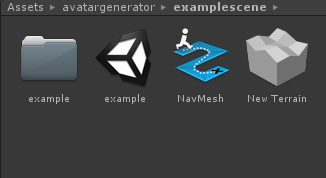
\includegraphics{0}
~\\ 

In case you want to add the personality demonstrator later on, or do not wish to restructure your entire scene, follow these steps.

\subsection{Import the Unity Package}
Naturally, the first step is to import the Personality Demonstrator Unity Package. %WHERE TO DOWNLOAD
You can choose to leave out our boilerplate models and animations if you want use your own instead.

\newpage
\subsection{Create a navmesh}
Our NPC's use Unity's Navmesh functions to move around your scene, so you need to define a terrain including a navmesh for them to walk around on. (A tutorial for this can be found here, in case you are not familiar with it: https://docs.unity3d.com/Manual/nav-BuildingNavMesh.html)

~\\
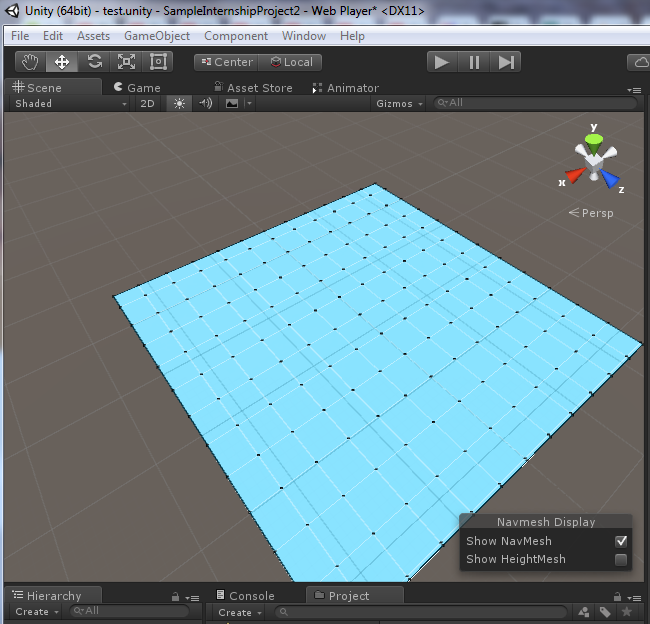
\includegraphics{1}
~\\ 
Above you can see what the end result should look like.

\newpage
\subsection{Add the AvatarGenerator Prefab to the project hierarchy}
This speaks for itself; This prefab needs to be added to the hierarchy in order to allow several important scripts, as well as the 'World' script, consisting of compiled Casanova code, to run.

~\\
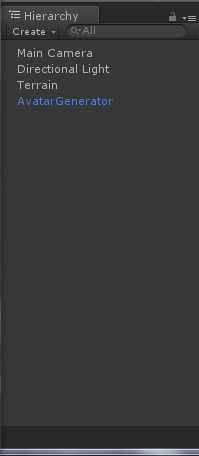
\includegraphics{2}
~\\ 

\newpage
\section{Configuration}
\subsection{Creating custom NPC's}
\subsubsection{Adding a fixed-value NPC}
If you want to add an NPC with fixed instead of random personality values, follow these steps:

\begin{enumerate}
\item Create a new Prefab and add the NpcObject script and an Animation component, containing a standard idle animation and a list of the animations that you want your NPC to be able to execute (More on this later, when we explain how to add custom animations.)
\item Add a new entry in Resources/players.xml for the new player you just made. 
\end{enumerate}
~\\
Your player object and players.xml ought to look something like this when you are done:

\begin{figure}[h]
\makebox[\textwidth]{%
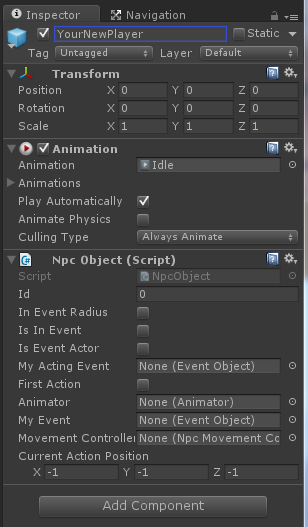
\includegraphics[width=0.49\textwidth, height=10cm]{8}%
\hfill    
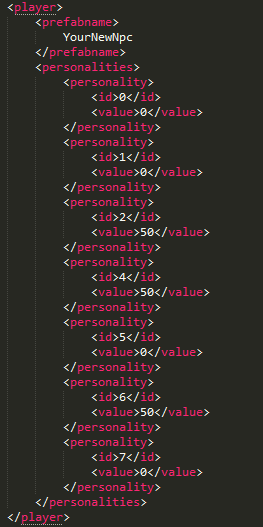
\includegraphics[width=0.49\textwidth, height=10cm]{7}%
}
\end{figure}

\newpage
\subsubsection{Adding a random-value NPC}
Adding an NPC whose personality values will be determined randomly is very easy; Simply follow these 2 steps.

\begin{enumerate}
\item Create a new Prefab \footnote{The easiest way to do this is to drag one of our pre-made Npc's into the hierarchy, changing what you want, and then dragging the finished NPC back to the Resources/ folder.} and add the NpcObject script and an Animation component, containing a standard idle animation and a list of the animations that you want your NPC to be able to execute (More on this later, when we explain how to add custom animations.) \footnote{This is done in the same way as with a fixed-value NPC} 
\item Add a new entry in settings.xml for the new NPC's you just made, supplying only the name of the NPC's gameObject.
\end{enumerate}

~\\
Your player object and players.xml ought to look something like this when you are done:

\begin{figure}[h]
\makebox[\textwidth]{%
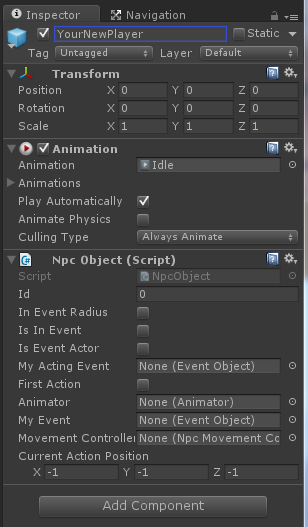
\includegraphics[width=0.49\textwidth, height=9cm]{8}%
\hfill    
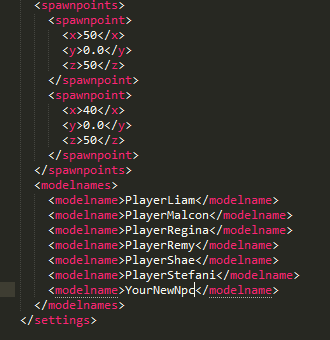
\includegraphics[width=0.49\textwidth, height=9cm]{9}%
}
\end{figure}

\newpage
\subsection{Customizing available NPC traits}
You can create your own personality traits, and determine how they can be set in the Unity Editor. 

\subsubsection{Defining personality traits in XML or via the Unity Interface}
You can either define new personality traits in settings.xml, or via the Unity Interface.

~\\
If you uncheck the checkbox under 'Use default value' you can create new personalities in the following way:
Increase the amount of personalities; then, set the values of the new personality.

~\\
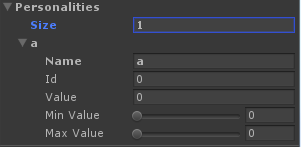
\includegraphics[]{16}

\subsubsection{Creating your own personality traits via XML}
If you check the checkbox under 'Use default value' you can create new personalities in this way:
Add a new personality tag and it's body in settings.xml. Note that the new trait has to have a unique ID. 

~\\
Also, note that the Personality's name tag is not used directly by the program; its' only use is to make it easier for you to see which personality id is representing which real-life trait.

~\\
Of course, in order for the personality to be actually used, you have to include it when creating a new personality for an NPC or when you are setting the personality values of an action. For example:

\begin{figure}[h]
\makebox[\textwidth]{%
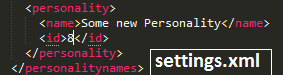
\includegraphics[width=0.49\textwidth, height=1.5cm]{10}%
\hfill    
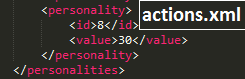
\includegraphics[width=0.49\textwidth, height=1.5cm]{11}%
}
\end{figure}

~\\
You can create, add and use as many personality values as you like! 

~\\
Personality values always range from 0 to 100.



\newpage
\subsubsection{Switching between random and fixed-value NPC's}
You can easily switch between using a fixed amount of fixed-value NPC's or using a variable amount of NPC's with random personality values in the Unity Editor. 

~\\
Just check the AvatarGenerator's 'Auto Generate Characters' value in order to use the fixed NPC's, or uncheck it and set the amount of random-personality NPC's that you want to create.

~\\
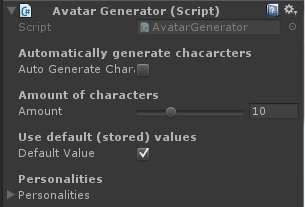
\includegraphics{12}

\newpage
\subsection{Creating custom actions and importing animations}
\subsubsection{Creating actions using the editor}
We created a simple actions editor in Python, which makes it very easy to create your own actions in a visual interface and to define their relationship to eachother.

~\\
You can find the executable at Assets/avatargenerator/grapheditor. 


~\\
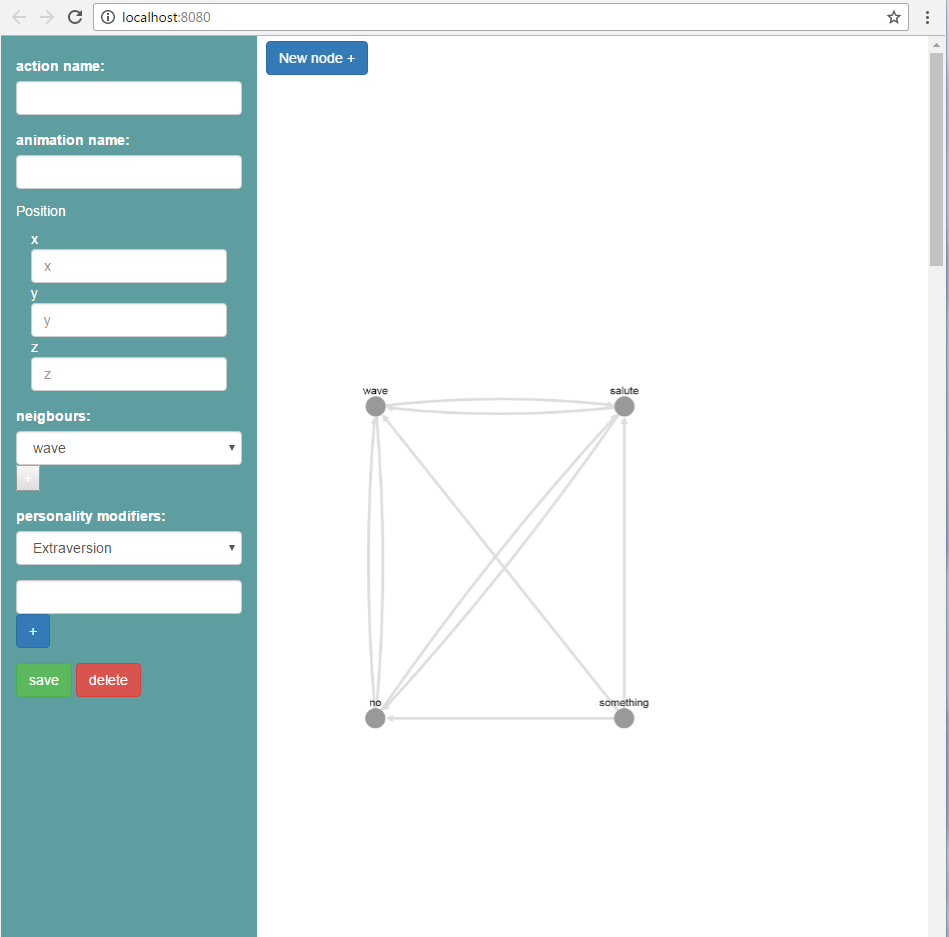
\includegraphics[scale=0.65]{14}

\newpage
\subsubsection{Creating actions manually}
A new action is easily defined using actions.xml.

~\\
Each action contains the following values in xml:

\begin{enumerate}
\item The actions that an NPC can choose when he/she is done with the selected action
\item The personality values of this action: The more these match with the NPC's personality values, the more likely the NPC will choose to perform this action.
\item The position of the action.
\item The id of the action.
\item The name of the action, which is only used for debugging purposes and to make reading this XML file easier for you.
\item The name of the animation tied to this action.
\end{enumerate}


\newpage
An example: 

~\\
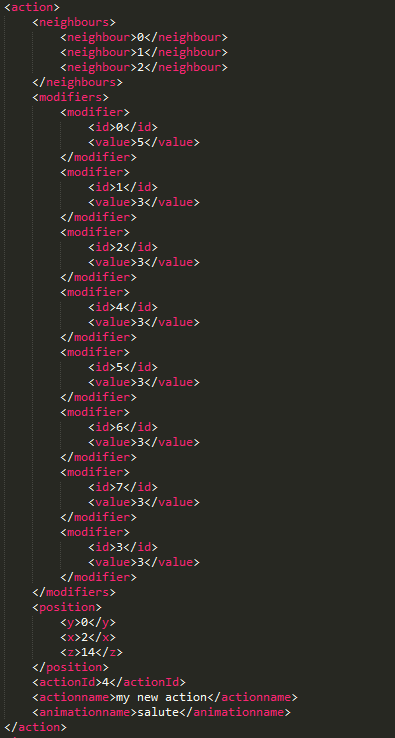
\includegraphics{13}

\newpage
\subsubsection{Importing animations for actions}
Of course, you can add your own animations to use in your custom actions. There are some prerequisites however;

\begin{enumerate}
\item Every animation must be in the .FBX format
\item Every animation has to have its' rig->Animation Type set to Legacy. 
\item The animation has to be added to in XML to the action that you wish to associate with it, as explained on the previous 2 pages
\item Last but not least, the animation has to be added to each NPC's list of possible animations. (The screenshot below shows where this can be done since it is not very obviously visible in the Unity Editor)
\end{enumerate}

~\\
Simply expand the animations tab, increment the animations number and select your animation in the new slot. Make sure your animations' name and the animation name that is used in your action in xml are exactly the same!

~\\
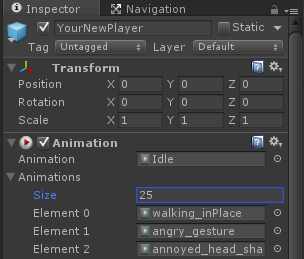
\includegraphics{15}


\end{document}
